We will investigate the dynamics of a glacier. Specifically the shape, size and internal movements are of interest.

We will assume that the glacier is situated along a valley with constant and relatively small incline $\alpha$. $x^*$ will denote the position along the length of this valley, and $z^*$ will denote the heigh perpendicular from the valley floor. We will also assume that the glacier behaves uniformly along its width, effectively ignoring the $y^*$-coordinate.

The $z^*$-coordinate of the glacier surface at time $t^*$ and position $x^*$ is given by $h^* = h^*(x^*, t^*)$. The point velocity of the glacier is denoted by $\vec{w}^* = (u^*, v^*)$, $u^*$ and $v^*$ being the $x^*$ and $z^*$ components, respectively.

This model is demonstrated in \figurename{ \ref{fig:coordinate_system}}.

\begin{figure}
  \centering
    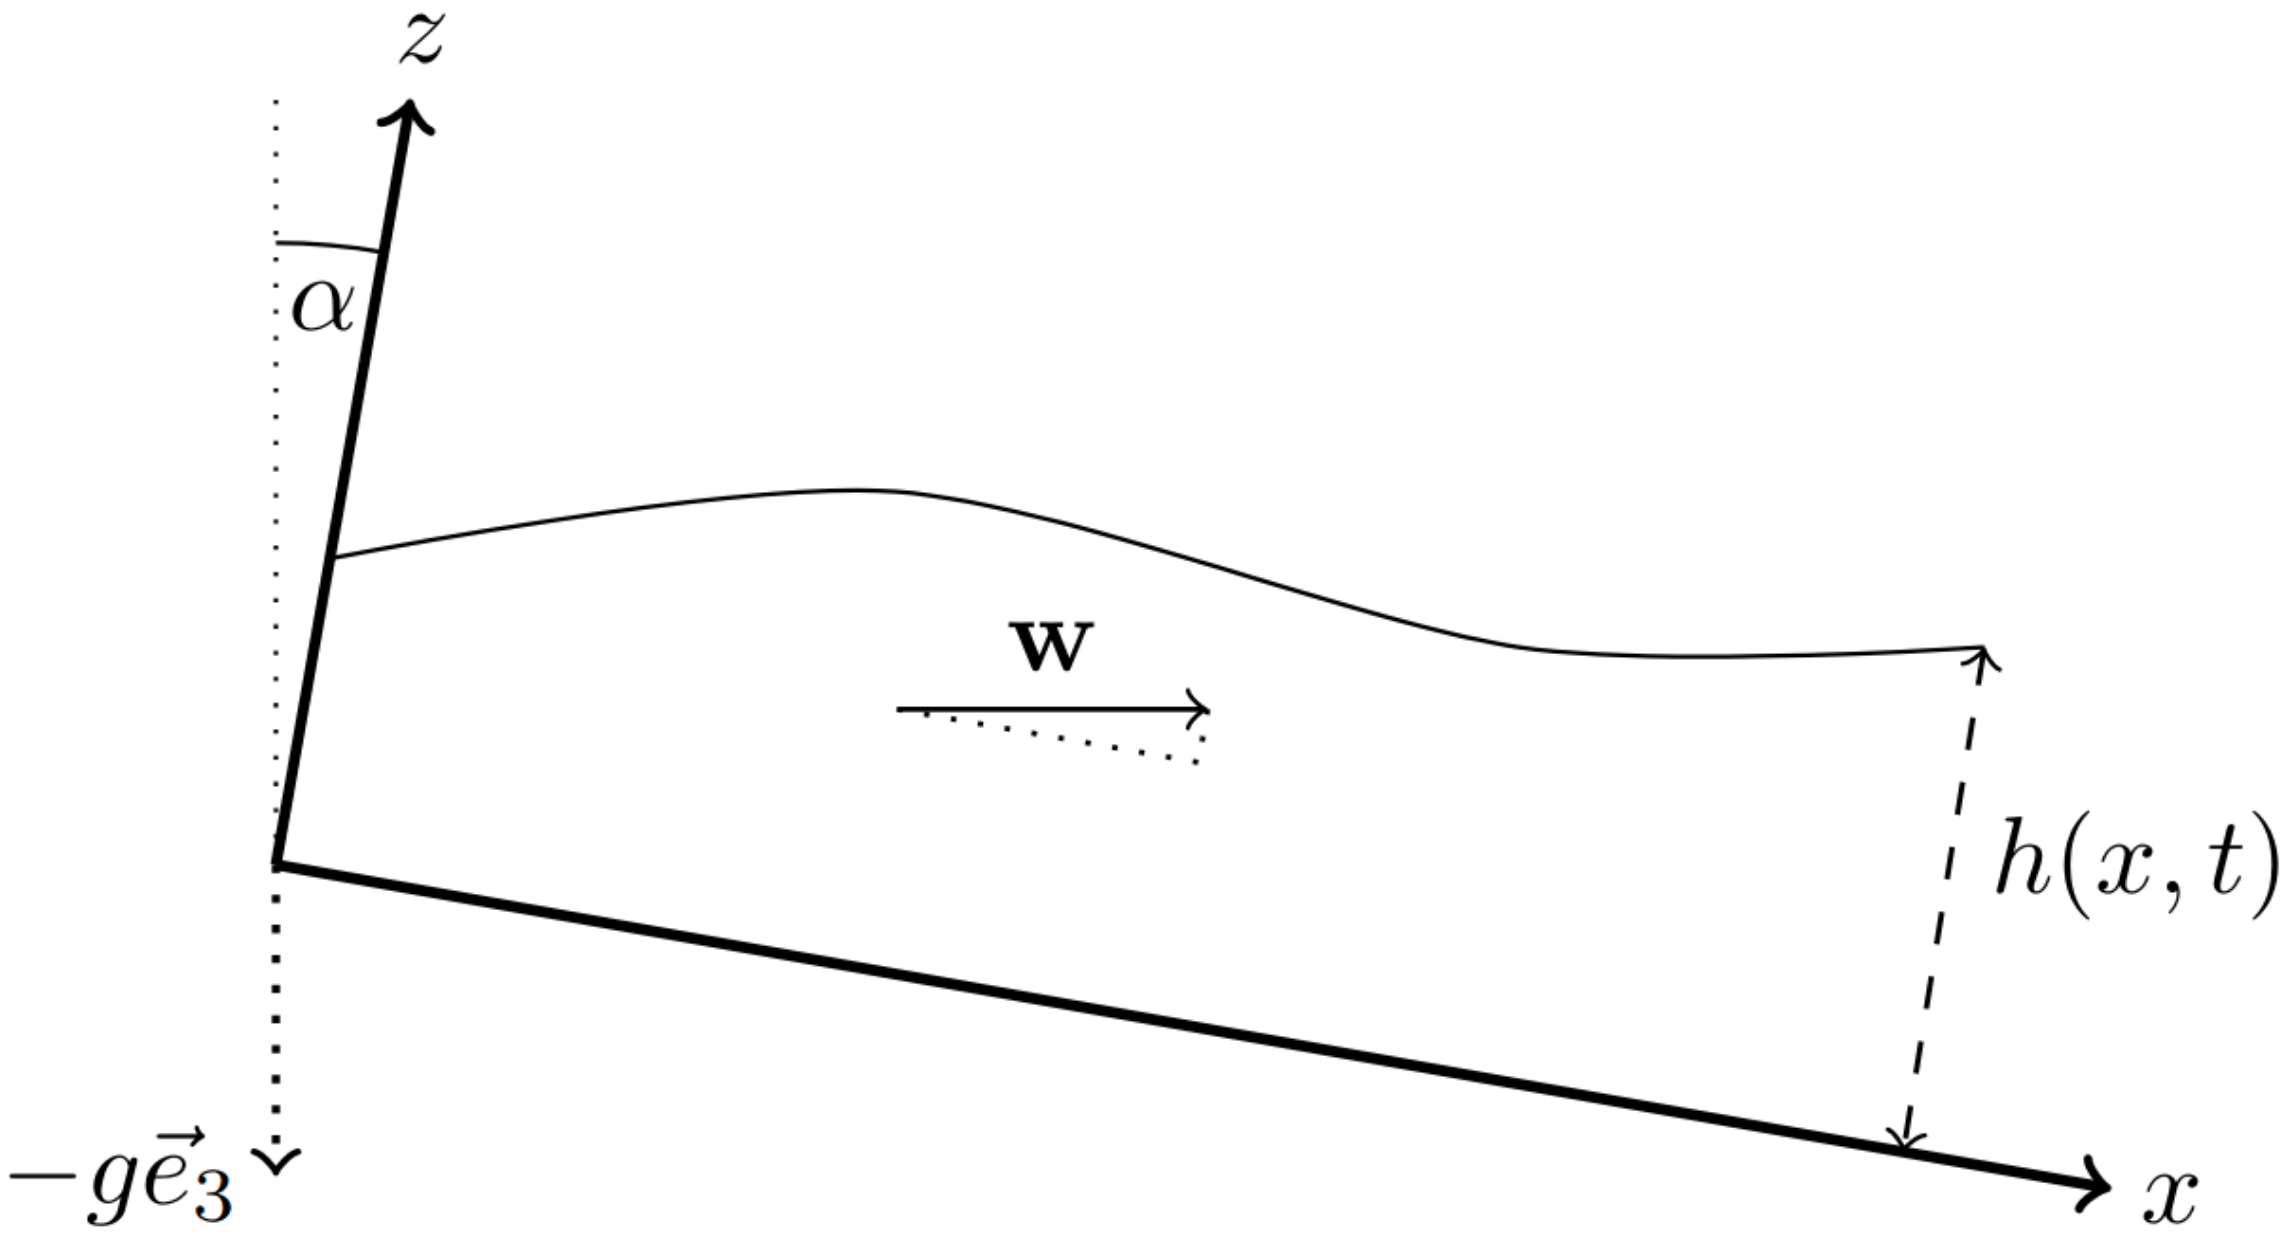
\includegraphics[width=0.5\textwidth]{images/coordinate_system.png}
  \caption{Sketch showing the coordinate system of the glacier. $\alpha$ denotes the slope of the valley floor, $h = h(x, t)$ the glacier's perpendicular height above the valley, and $\vec{w} = (u, v)$ its velocity in $x$ and $z$ directions, respectively \cite{project-description}.}
  \label{fig:coordinate_system}
\end{figure}

We will now formulate equations based on the conservation of mass and momentum in order to describe the relationship between the height of the glacier and the velocity within it.
